\documentclass{article}
\usepackage[utf8]{inputenc}
\usepackage{algorithm}
\usepackage{algorithmic}
\usepackage{amsfonts}
\usepackage{graphicx}
\usepackage{listings}
\usepackage{xcolor}
\usepackage{amsmath}
\usepackage{amsthm,amssymb}
\theoremstyle{definition}
\theoremstyle{theorem}
\usepackage{geometry}
\geometry{a4paper,left=25mm,right=25mm,bottom=25mm,top=25mm,footskip=10mm}
\newtheorem{definition}{Definíció}
\newtheorem{theorem}{Tétel}
\newtheorem{proof}{Bizonyítás}
\newtheorem{example}{Példa}
\renewcommand{\qedsymbol}{\rule{0.7em}{0.7em}}
\title{Szakdolgozat}
\author{Szabó Bence Dániel }
\date{Date}

\definecolor{codegreen}{rgb}{0,0.6,0}
\definecolor{codegray}{rgb}{0.5,0.5,0.5}
\definecolor{codepurple}{rgb}{0.58,0,0.82}
\definecolor{backcolour}{rgb}{0.95,0.95,0.92}

\lstdefinestyle{mystyle}{
    backgroundcolor=\color{backcolour},   
    commentstyle=\color{codegreen},
    keywordstyle=\color{magenta},
    numberstyle=\tiny\color{codegray},
    stringstyle=\color{codepurple},
    basicstyle=\ttfamily\footnotesize,
    breakatwhitespace=false,         
    breaklines=true,                 
    captionpos=b,                    
    keepspaces=true,                 
    numbers=left,                    
    numbersep=5pt,                  
    showspaces=false,                
    showstringspaces=false,
    showtabs=false,                  
    tabsize=2
}
\lstset{style=mystyle}
\begin{document}
\section{Bevezetés}
Itt van a bevezető szöveg
\section{Python nyelv}
\begin{center}
    
\includegraphics[width=\textwidth]{plots/python-logo.png}
    %https://www.python.org/static/community_logos/python-logo-master-v3-TM.png
\end{center}

A Python egy magas szintű programozási nyelv egy könnyen elsajátítható szintaxissal. Azért erre a nyelvre esett
a választásom, mert sok csomag elérhető hozzá, nagyon jól dokumentált, nem kell típusokat használni benne az 
esetek nagy többségében, nyílt és ebben dolgozom, ezért ezt ismerem a legjobban. \newline



A Python nyelvben zárójeleket igazából csak a függvények után a paraméter megadásoknál és az indexeléseknél szoktuk használni. Ez egy nagy különbség sok másik nyelvvel szemben, ahol a kódok különböző részeit zárójelekbe / kapcsoszárójelekbe kell írnunk. Itt a tabulátor lesz az elválasztó karakter a kódrészletek között.

A következőkben nézzünk meg néhány nyelv specifikus dolgot, amelyeket a szakdolgozat további részében felhasználunk.

\subsection{Python függvények}
Pythonban minden függvényt a \textit{def} szóval kezdünk, amit a függvény neve követ, majd zárójelek közé beírjuk a paramétereket és vesszővel választjuk el, ha vannak. A csukó zárójel után mindig ki kell tenni a kettőspontot. Ezután a következő sorban kell folytatnunk a kódot, de egy tabulátornyi hellyel jobbrább, mint ahogy a \textit{def} szócskát elhelyeztük.
\lstinputlisting[language=Python]{python-bevezetohoz-scriptek/function_template.py}
A függvény paramétereinél nem szükséges, hogy megadjuk milyen típusú inputot vár el, azonban a saját segítségünkre megadhatjuk ezeket a következő képpen: a paraméter neve után kettőspontot írunk, majd az adattípus nevét, pl. str, mint String, dict, mint Dictionary, int, mint integer, stb...
\lstinputlisting[language=Python]{python-bevezetohoz-scriptek/typing_template.py}

A függvény visszatérési értékét pedig a \textit{return} szó után adhatjuk meg, amennyiben szükség van rá
\subsection{Ciklusok}
\subsubsection{For ciklus}
A \textit{for} ciklus ebben a nyelvben nagyon hasonlít más nyelvek \textit{for each} megoldásaira, mert a for mindig valamilyen listán iterál végig, legyenek azok számok vagy egyéb objektumok. A szintaxisa a következő :
A \textit{for} szó után megadjuk a változót, amit használunk az iterálás alatt, majd az \textit{in} szó után megadjuk a sorozatot, amin végiglépkedünk. A végére itt is kettőspontot kell raknunk, akárcsak a függvényeknél
\pagebreak
\lstinputlisting[language=Python]{python-bevezetohoz-scriptek/for_template.py}

\subsubsection{While ciklus}
A while ciklust hasonlóan adjuk meg , mint más nyelvekben. A \textit{while} szó után jön az eldöntendő feltétel, és ameddig a feltétel igaz, addig a blokkban lefog futni a kódrészlet. A feltétel végét itt is kettősponttal zárjuk le.
\lstinputlisting[language=Python]{python-bevezetohoz-scriptek/while_template.py}
\subsection{PEP8}
**kódformázási útmutató**

\subsection{Python csomagok}
Mint minden nyelvben, itt is tudunk importálni már készen levő csomagokat, amelyek tartalmaznak a célnak megfelelő osztályokat, azon belül metódusokat és egyéb hasznos dolgokat. Ha nincs feltelepítve a csomag, akkor a \textbf{pip install csomag-neve} paranccsal tehetjük meg azt.
Amint ezt megtettük, az \textit{import csomag-neve as alias-csomag-neve} módon importálhatjuk a kódunkba. A könnyebb olvashatóság érdekében szokás \textit{alias}-t használni, de nem szükséges.

\lstinputlisting[language=Python]{python-bevezetohoz-scriptek/import_template.py}
\section{Numerikus integrálás}
A numerikus integrálás nagyon fontos része a numerikus módszereknek. Egyrészről gyorsabban megkaphatjuk a határozott  integrál értékét, másrésszről vannak olyan függvények, amelyeknek nem tudjuk kiszámolni papíron az integrál értéket, csak becsülni tudjuk alulról és/vagy felülről.

\begin{definition}
Lagrange-féle interpolációs polinom

Ezt még meg kell írni + nézd meg az opkut3-as dolgokat!
\end{definition}
A numerikus integrálás nagyban támaszkodik a kvadratúra képletekre.
\begin{definition}
Kvadratúra képletek általánosan

Az integrál értékét tudjuk közelíteni az ún. \textit{Kvadratúra képlettel}.\newline 
\begin{equation*}
    \int_{a}^{b} f(x) dx \approx \sum_{k = 0}^{n} c_k f(x_k) = \sum_{k=0}^n \sigma_k
\end{equation*}
 , ahol $x_i \in [a,b]$
\end{definition}

Most nézzünk meg néhány kvadratúra képletet.
\subsection{Newton - Cotes formula}


Az integrálni való halmazt osszuk fel egyforma hosszúságúra, így vegyünk ekvidisztáns alappontokat.
$x_k = a + hk $, ahol $k=0,1,...,n$ , $h = \frac{b-a}{n}$

Írjuk fel az interpolációs kvadratúra képletet.
\newline
\begin{equation*}
    c_k = \int_a^{b} l_k(x) dx = h \int_0^{n} l_k (a+ht) dt = \frac{b-a}{n} \int_0 ^{n} \Pi_{j=0, j \neq k}^n \frac{t-j}{k-j} dt = \frac{b-a}{n} \frac{1}{k! (n-k)!} \int_0^n \Pi_{j=0}^{k-1} (t-j) \Pi_{j=k+1}^{n} (j-t) dt


\end{equation*}

\subsection{Összetett kvadratúra képlet}

\begin{equation*}
 \int_a^{b} f(x) dx = \sum_{j = 1} ^{m} \int_{a_{j-1}} ^{a_j} f(x) dx 
\end{equation*}
 ahol $a_0 = a, a_m =b $  

A baloldali részintegrált írjuk fel az interpolációs kvadratúra képlettel:
\begin{equation*}
\int_{a_{j-1}}^{a_j} f(x) dx \approx \sum_{k=0}^{r} c_{k,j}f(x_{k,j})
\end{equation*}

Innen helyettesítsünk vissza az eredeti képletbe
\begin{equation*}
\int_a^b f(x) dx \approx \sum_{j=1}^{m} \sum_{k=0}^{r} c_{k,j} f(x_{k,j})
\end{equation*}


\subsection{Érintő formula}

Az érintő formulához felfogjuk használni a függvények lineáris Taylor közelítését. Ezen felül vegyük az intervallum ekvidisztáns felosztását.
\begin{equation*}
   x_k = a + (k - \frac{1}{2})h  
\end{equation*}
, ahol $h = \frac{b-a}{n}, k =1,...,n$. 


A Taylor közelítése a függvénynek a $[x_k-\frac{h}{2},x_k+\frac{h}{2}]$ intervallumon
\begin{equation*}
    f(x) \approx f(x_k)+f'(x_k)(x-x_k).
\end{equation*}

\begin{equation*}
   
\int_{x_k-\frac{h}{2}}^{x_k + \frac{h}{2}} \approx \int_{x_k - \frac{h}{2}}^{x_k + \frac{h}{2}} [f(x_k) + f'(x_k)(x-x_k)] dx = hf(x_k)
\end{equation*}
\newline
Innen pedig kapjuk, hogy
\begin{equation*}
\int_a^b = f(x) dx = \sum_{k=1}^n \int_{x_k - \frac{h}{2}}^{x_k + \frac{h}{2}} f(x)dx \approx h \sum_{k=1}^n f(x_k)
\end{equation*}

\textbf{Ide rakd be az érintős-integrálós rajzot}

\subsection{A trapéz módszer és a Newton - Cortes módszer}
Írjuk fel a Newton - Cortes formulát n = 1 és k = 0 melett:
\begin{equation*}
c_0 = \frac{b-a}{1} \frac{1}{0!(1-0)!} \int_0^{1} \Pi_{j=0}^{0-j} \Pi_{j=0+1}^{1} (j-t) dt = (b-a) \int_0^1 (1-t) dt = \frac{b-a}{2}
\end{equation*}

\begin{equation*}
c_1 = \frac{b-a}{2}
\end{equation*}
Ekkor 

\begin{equation*}
    \int_a^b f(x) dx \approx \frac{b-a}{2}[f(a) + f(b)] = \sum_{k=0}^{1} \frac{b-a}{2} f(x_k), 
\end{equation*}
ahol $x_0 = a,x_1=b$
Ez pedig pont a trapéz területe! Nézzünk erre egy példát :
\newline

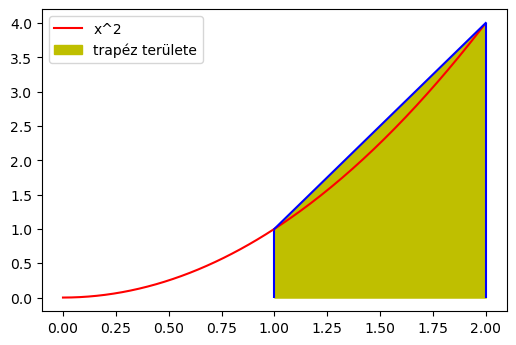
\includegraphics{plots/trapez_with_area.png}

Az integrál értéke ezen az intervallum 7/3. 
\begin{center}
$\int_{1}^{2} x ^2 dx = \frac{7}{3}$
\end{center}
Azonban, ha a ezen paraméterek között végezzük el a trapéz - területszámítást akkor 2.5 - t kapunk eredményként. Ezt onnan is láthatjuk, hogy a fenti ábrán a kék és piros vonal között még akad zöld terület. Azonban most számoljuk ki ezzel a módszerrel az integrál értékét az [1,1.5] és [1.5,2] intervallumokon. Ekkor eredményül 0.8125 és 1.5625, összesen 2.375 értéket kapunk, ami közelebb van a 7/3-hoz

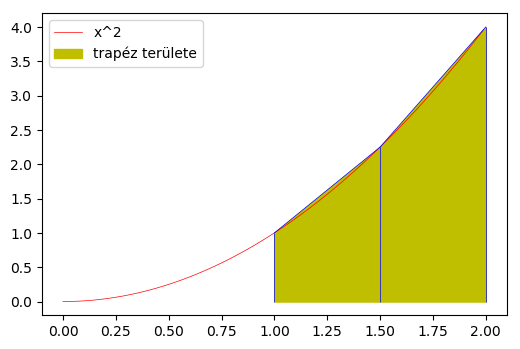
\includegraphics{plots/trapez_n=2.png}

\begin{definition}
Legendre polinom
[...]
\end{definition}
\begin{definition}
Gauss - féle kvadratúra összegek
\end{definition}

\subsection{Python kódok a fejezethez (saját , legyen SciPy?)}
\lstinputlisting[language=Python]{functions.py}
\subsection{Feladatmegoldások}

\section{Fokozatos közelítések módszere}
\begin{definition}{Lipschitz folytonosság}

\end{definition}
\begin{definition}{ODE}

\end{definition}

\begin{definition}Autonóm differenciál egyenlet

\end{definition}

\begin{definition}Lineáris differenciál egyenlet

\end{definition}

\begin{definition}Nem lineáris differenciál egyenlet

\end{definition}

\begin{definition}Homogén differenciál egyenlet

\end{definition}
\begin{definition}Nem homogén differenciál egyenlet

\end{definition}
\begin{definition}[Kezdetiérték-feladat]

\end{definition}
\begin{theorem}[Banach-féle fixponttétel]

\end{theorem}
%https://en.wikibooks.org/wiki/Ordinary_Differential_Equations/The_Picard–Lindelöf_theorem
\begin{theorem} [Picard - Lindenlöf]\\


Legyen I =[a,b] egy intervallum , és egy f függvény,

\[
f :  I \times \mathbb{R}^n \rightarrow \mathbb{R}^n f

\]
Legyen x' pedig egy ODE
\[
x'(t) = f(t,x(t))
\]
Ha f Lipschitz folytonos x(t)-ben, akkor az ODE-nek létezik egyértelmű megoldása [a,a + $\epsilon$] 
intervallumon minden 
\[
x(0) = x_0 \in \mathbb{R}^n, \epsilon < \frac{1}{L}
\] halmazra és L pedig x(t) Lipschitz konstansa
\end{theorem}
\begin{proof}
Írjuk fel ezt egy kezdeti-érték feladatra 
\begin{equation*}
    \begin{cases}
       f :  I \times \mathbb{R}^n \rightarrow \mathbb{R}^n , t \in [a,a + \epsilon]\\
       x'(t) = f(t,x(t))\\
    \end{cases}       
\end{equation*}

Ez a Newton - Leibniz tétel miatt pedig erre az alakra hozható:
\begin{equation*}
    \forall t \in [a, a +\epsilon] : x(t) = x_0 + \int_{a}^{t} f(s,x(s)) ds
\end{equation*}
 ahol pedig $\epsilon < \frac{1}{L}$. Eszerint x(t) fixpontja a következő függvénynek : 
 
 \begin{equation*}
     T : \mathcal{C}([a, a +\epsilon]) \rightarrow \mathcal{C}([a, a +\epsilon]), T(x,t) := x_0 + \int_a^t f(s,x(s)) ds
 \end{equation*}
 T kielégíti a Lipschitz folytonosságot, mivel
 \begin{equation*}
    \begin{split}
     \lVert T(x,t) - T(y,t) \rVert =\lVert \int_a^t f(s,x(s)) ds - \int_a^t f(s,x(s)) ds \rVert &
     \leq \int_a^t \lVert f(s,x(s)) - f(s,y(s)) \rVert ds \leq \int_a^t L \lVert x(s) - y(s) \rVert &
     \leq (t-a) L \lVert x-y\rVert_{\infty} \leq \epsilon L \lVert x - y \rVert_{\infty}
     \end{split}
 \end{equation*}
 
 Ezt pedig nem értem teljesen: then 
T is a contraction, and hence the Banach fixed-point theorem is applicable, giving us both existence and uniqueness.
\end{proof}
\begin{definition}[Szubszcesszív approximációs módszer]
Vegyük a következő kezdetiérték problémát
\begin{equation*}
    \begin{cases}
       x'(t) = f(t,x(t))\\
       x(a) = b
    \end{cases}       
\end{equation*}
Fentebb tárgyaltuk a Picard-Lindelöf tételnél, hogy a Newton - Leibniz tétel miatt fennáll a következő
egyenlőség: \newline
\begin{equation*}
    x(t) = x(0) + \int_a^x f(t,x(t)) dt
\end{equation*}
Ekkor vegyük az \[x_0(l) = b\] állandót, majd kezdjünk el előre iterálni a következő képlet alapján:
\begin{equation*}
    x_{n + 1}(l) = b + \int_a^x f(t,x_n(t)) dt 
\end{equation*}
\end{definition}

\begin{example}[Exponenciális függvény]
\begin{equation*}
    \begin{cases}
       y'(t) = y\\
       y(0) = 1
    \end{cases}       
\end{equation*}
Kezdjünk el lépkedni.
\begin{equation*}
    y_1(x) = 1 + \int_0^x 1 dt = 1 + x
\end{equation*}
\begin{equation*}
    y_2(x) = 1 + \int_0^x 1+t dt = 1 + x + \frac{x^2}{2}
\end{equation*}
\begin{equation*}
    y_{\infty}(x) = exp(x)
\end{equation*}
\end{example}
\lstinputlisting[language=Python]{fokozatos_kozelitesek/subscessive.py}
\subsection{RK4}
\end{document}
